
\section{Benefits of open source and open science}
\topicFramePrimary{Let's work collectively and co-develop open-source software}
% \topicFramePrimary{
\includegraphics[width=0.5\textwidth]{openptv}}

\begin{frame}[label=opensource-0]{The most important benefit of open source is sustainability}

\begin{card}[It is a community thing]
\begin{itemize}
\item Developing real-time 3D-PTV as an open-source project: increased collaboration and sharing of knowledge. 
\item You meet great people along the way.
\item The open-source approach has been successful in other scientific fields: ML/AI, PyData, OpenCV, OpenFOAM, etc.
\item There are challenges in developing an open-source real-time 3D-PTV project: consistency, documentation, and funding.
\end{itemize}
\end{card}
\end{frame}


\begin{frame}[label=opensource-1]{Use sustainable software: Python, NumPy, PyData, Github}
\begin{columns}
\column{.4\textwidth}
    \centering 
\includegraphics[width=0.9\textwidth]{openptv}
     
     
\includegraphics[width=.9\textwidth]{pyptv} 
     
     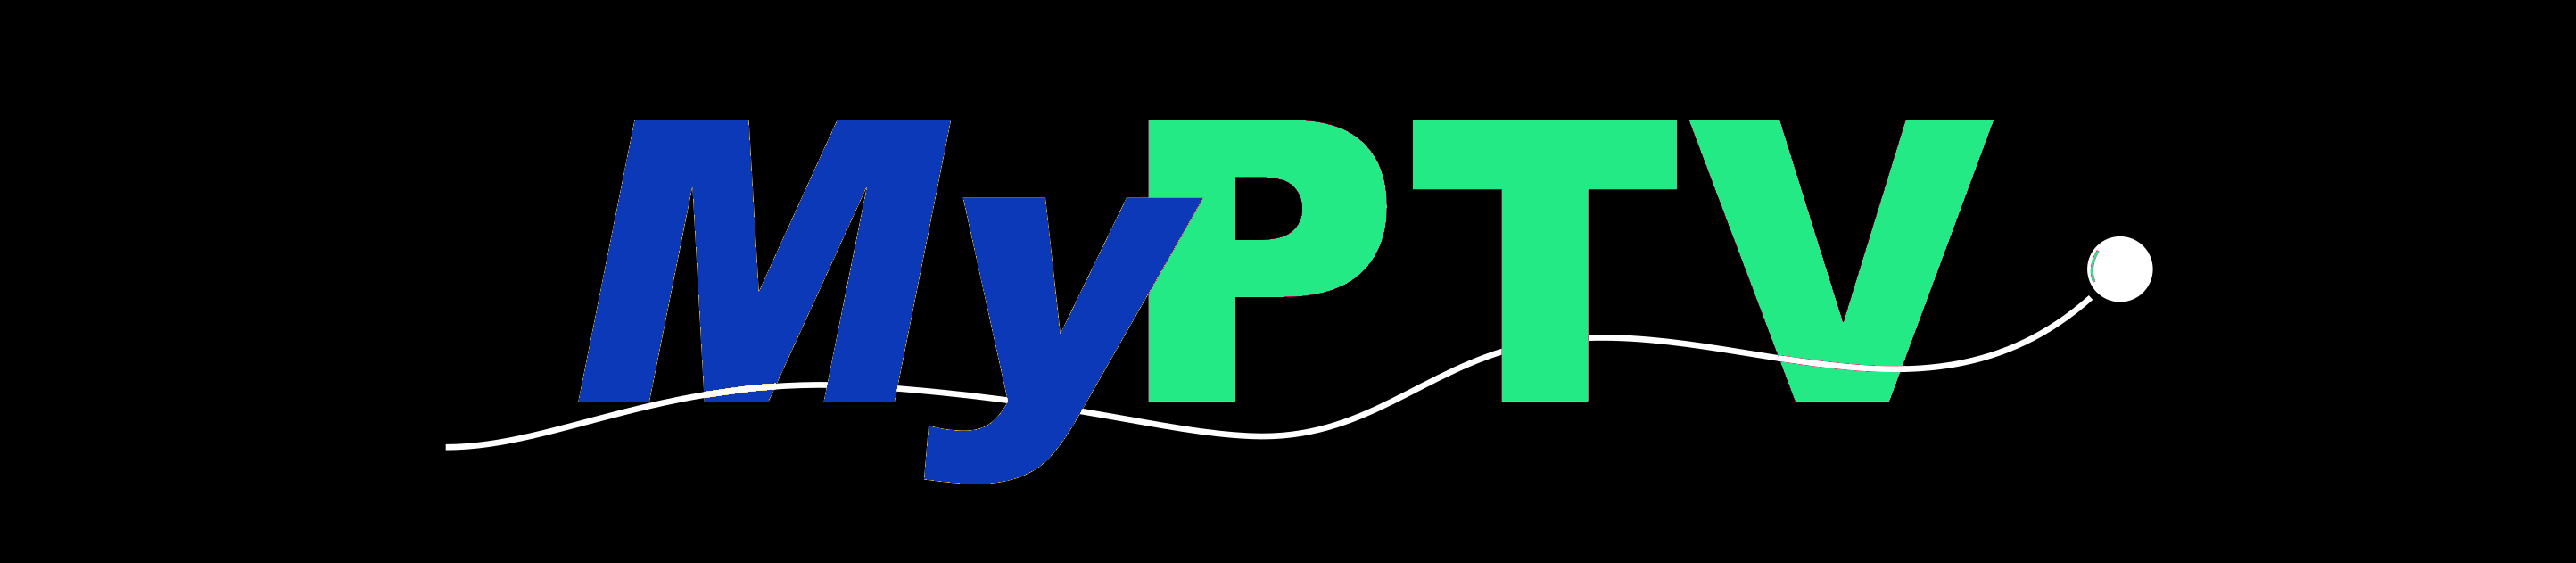
\includegraphics[width=.9\textwidth]{fig/myptv_logo.png}

\column{.65\textwidth}
\begin{card}[Plus many more:]
    \begin{itemize}
    \item FlowTracks - trajectories database management, Yosef Meller, TAU
    \item BlobRecorder - 1Vision LTD 
    \item Lagrangian plotting library, Ron Shnapp, BGU
    \item Virtual 3D-PTV Alex Ruiz, Samik Bhattacharya, UCF
    \end{itemize}
\end{card}
\end{columns}
\end{frame}



\section{Take home message}\label{sec:summary}

\begin{frame}{Closing thoughts}

Real-time 3D particle tracking velocimetry (3D-PTV) provides numerous advantages for fluid flow measurement and analysis, including:

\begin{itemize}
\item Immediate feedback on the velocity field
\item Faster decision-making
\item Improved accuracy and precision of measured data
\item Detailed insight into fluid dynamics
\item Real-time issue detection and troubleshooting
\end{itemize}

Real-time 3D-PTV is an invaluable tool for a wide range of applications, from fundamental fluid dynamics research to industrial process optimization and safety-critical applications.

\end{frame}


\begin{frame}{Take-home message}
  \begin{itemize}
  \item Real-time image analysis on FPGA is feasible for long-recording, high-speed 3D-PTV
  \item Real-time feature changes a paradigm about 3D-PTV: from the laboratory, table-top experiments to wind tunnel, field experiments, and new applications (e.g. control)
  \item Instead of dense field representation (TomoPIV, Shake the box),  you can obtain an unprecedented data set of of Lagrangian trajectories, reducing particle density and gaining new features like infinitely long time recording, along with Lagrangian velocity fields and material derivatives. 
  \end{itemize}
  
  \begin{cardTiny}\href{https://www.nature.com/articles/s41598-019-43555-2}{Details are in ``Extended 3D-PTV ...'' by Shnapp et al. Sci. Rep.}
  \end{cardTiny}
  
  \end{frame}
  
  \begin{frame}{Towards a real real-time 3D-PTV :) \href{https://www.dropbox.com/s/os4tz91gq0ginp8/real_time_3dptv_calibration.mp4?raw=1}{\ldots}}
  \embedvideo{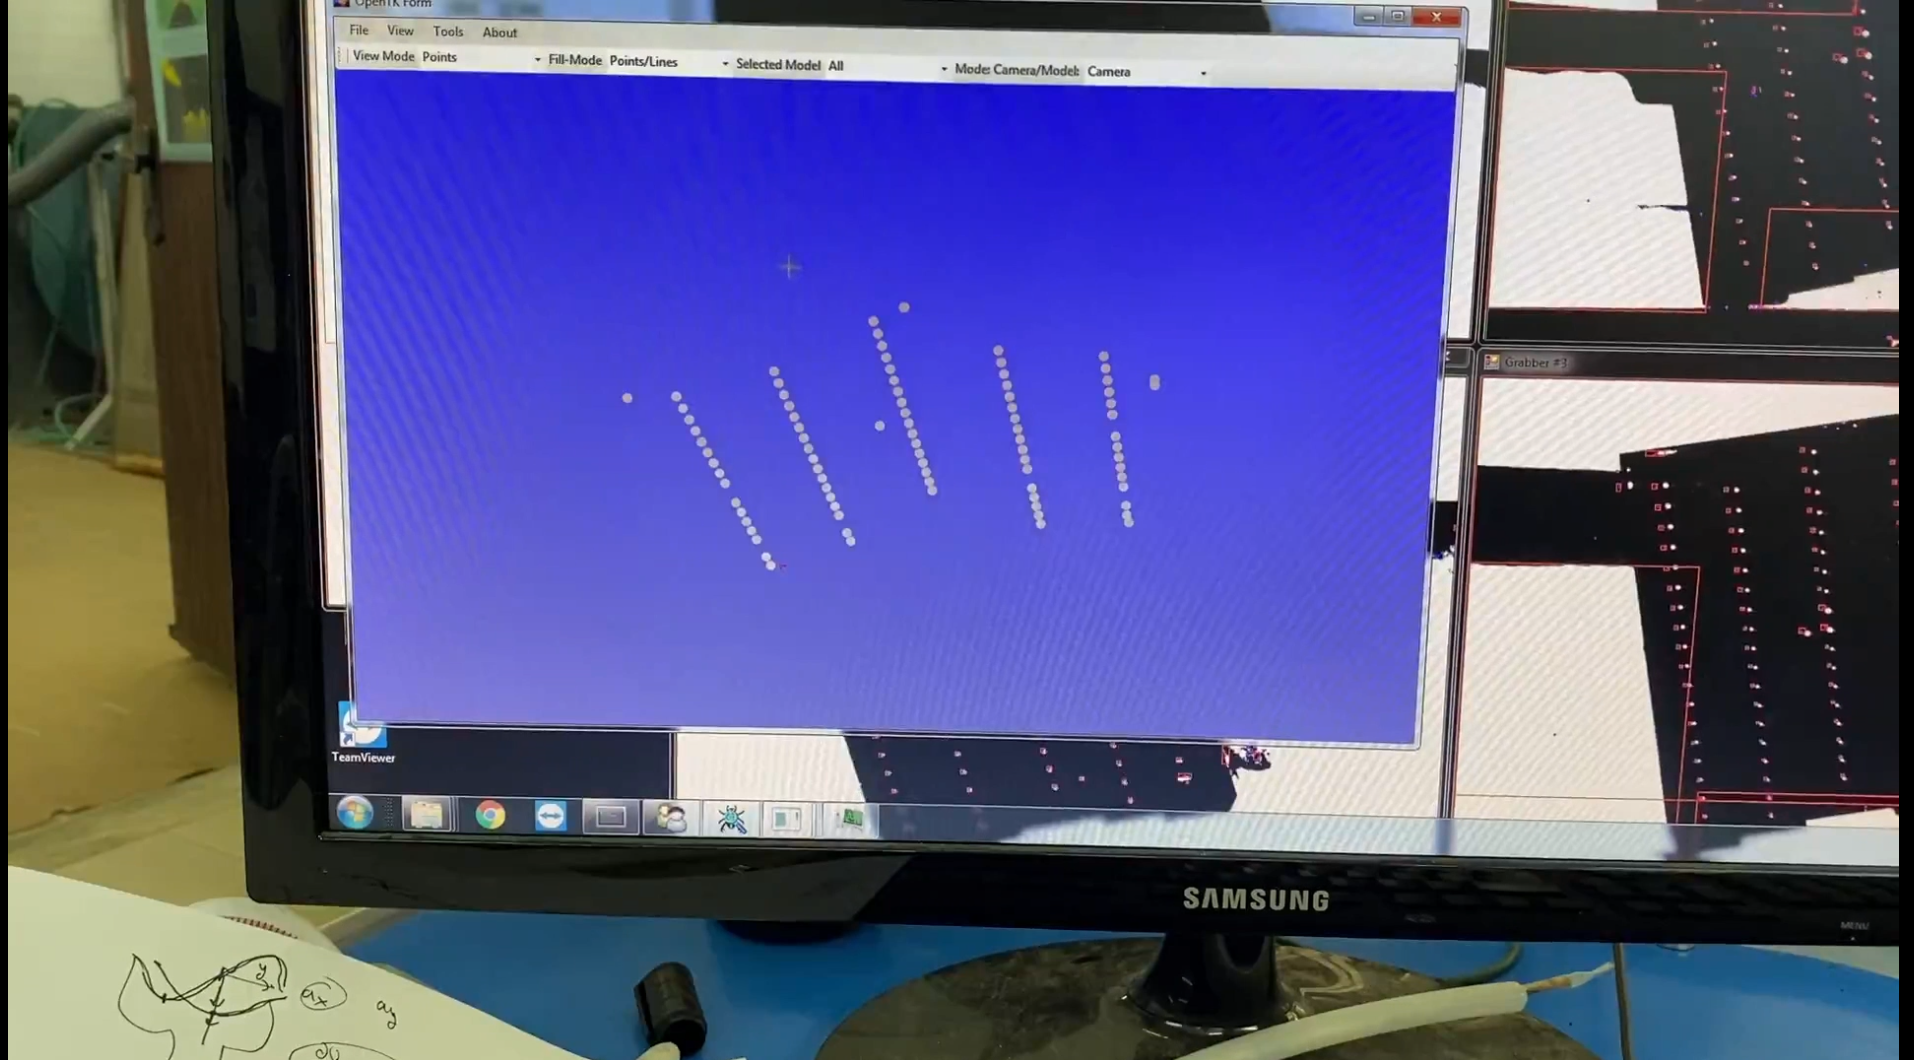
\includegraphics[width=0.9\textwidth]{fig/real_time_3dptv_calibration.png}}{video/real_time_3dptv_calibration.mp4}    
  \end{frame}

  
  \begin{frame}{Thanks for your attention) \href{https://www.dropbox.com/s/resn98zu5l7vtty/real_time_3dptv.mp4?raw=1}{\ldots}}
  \embedvideo{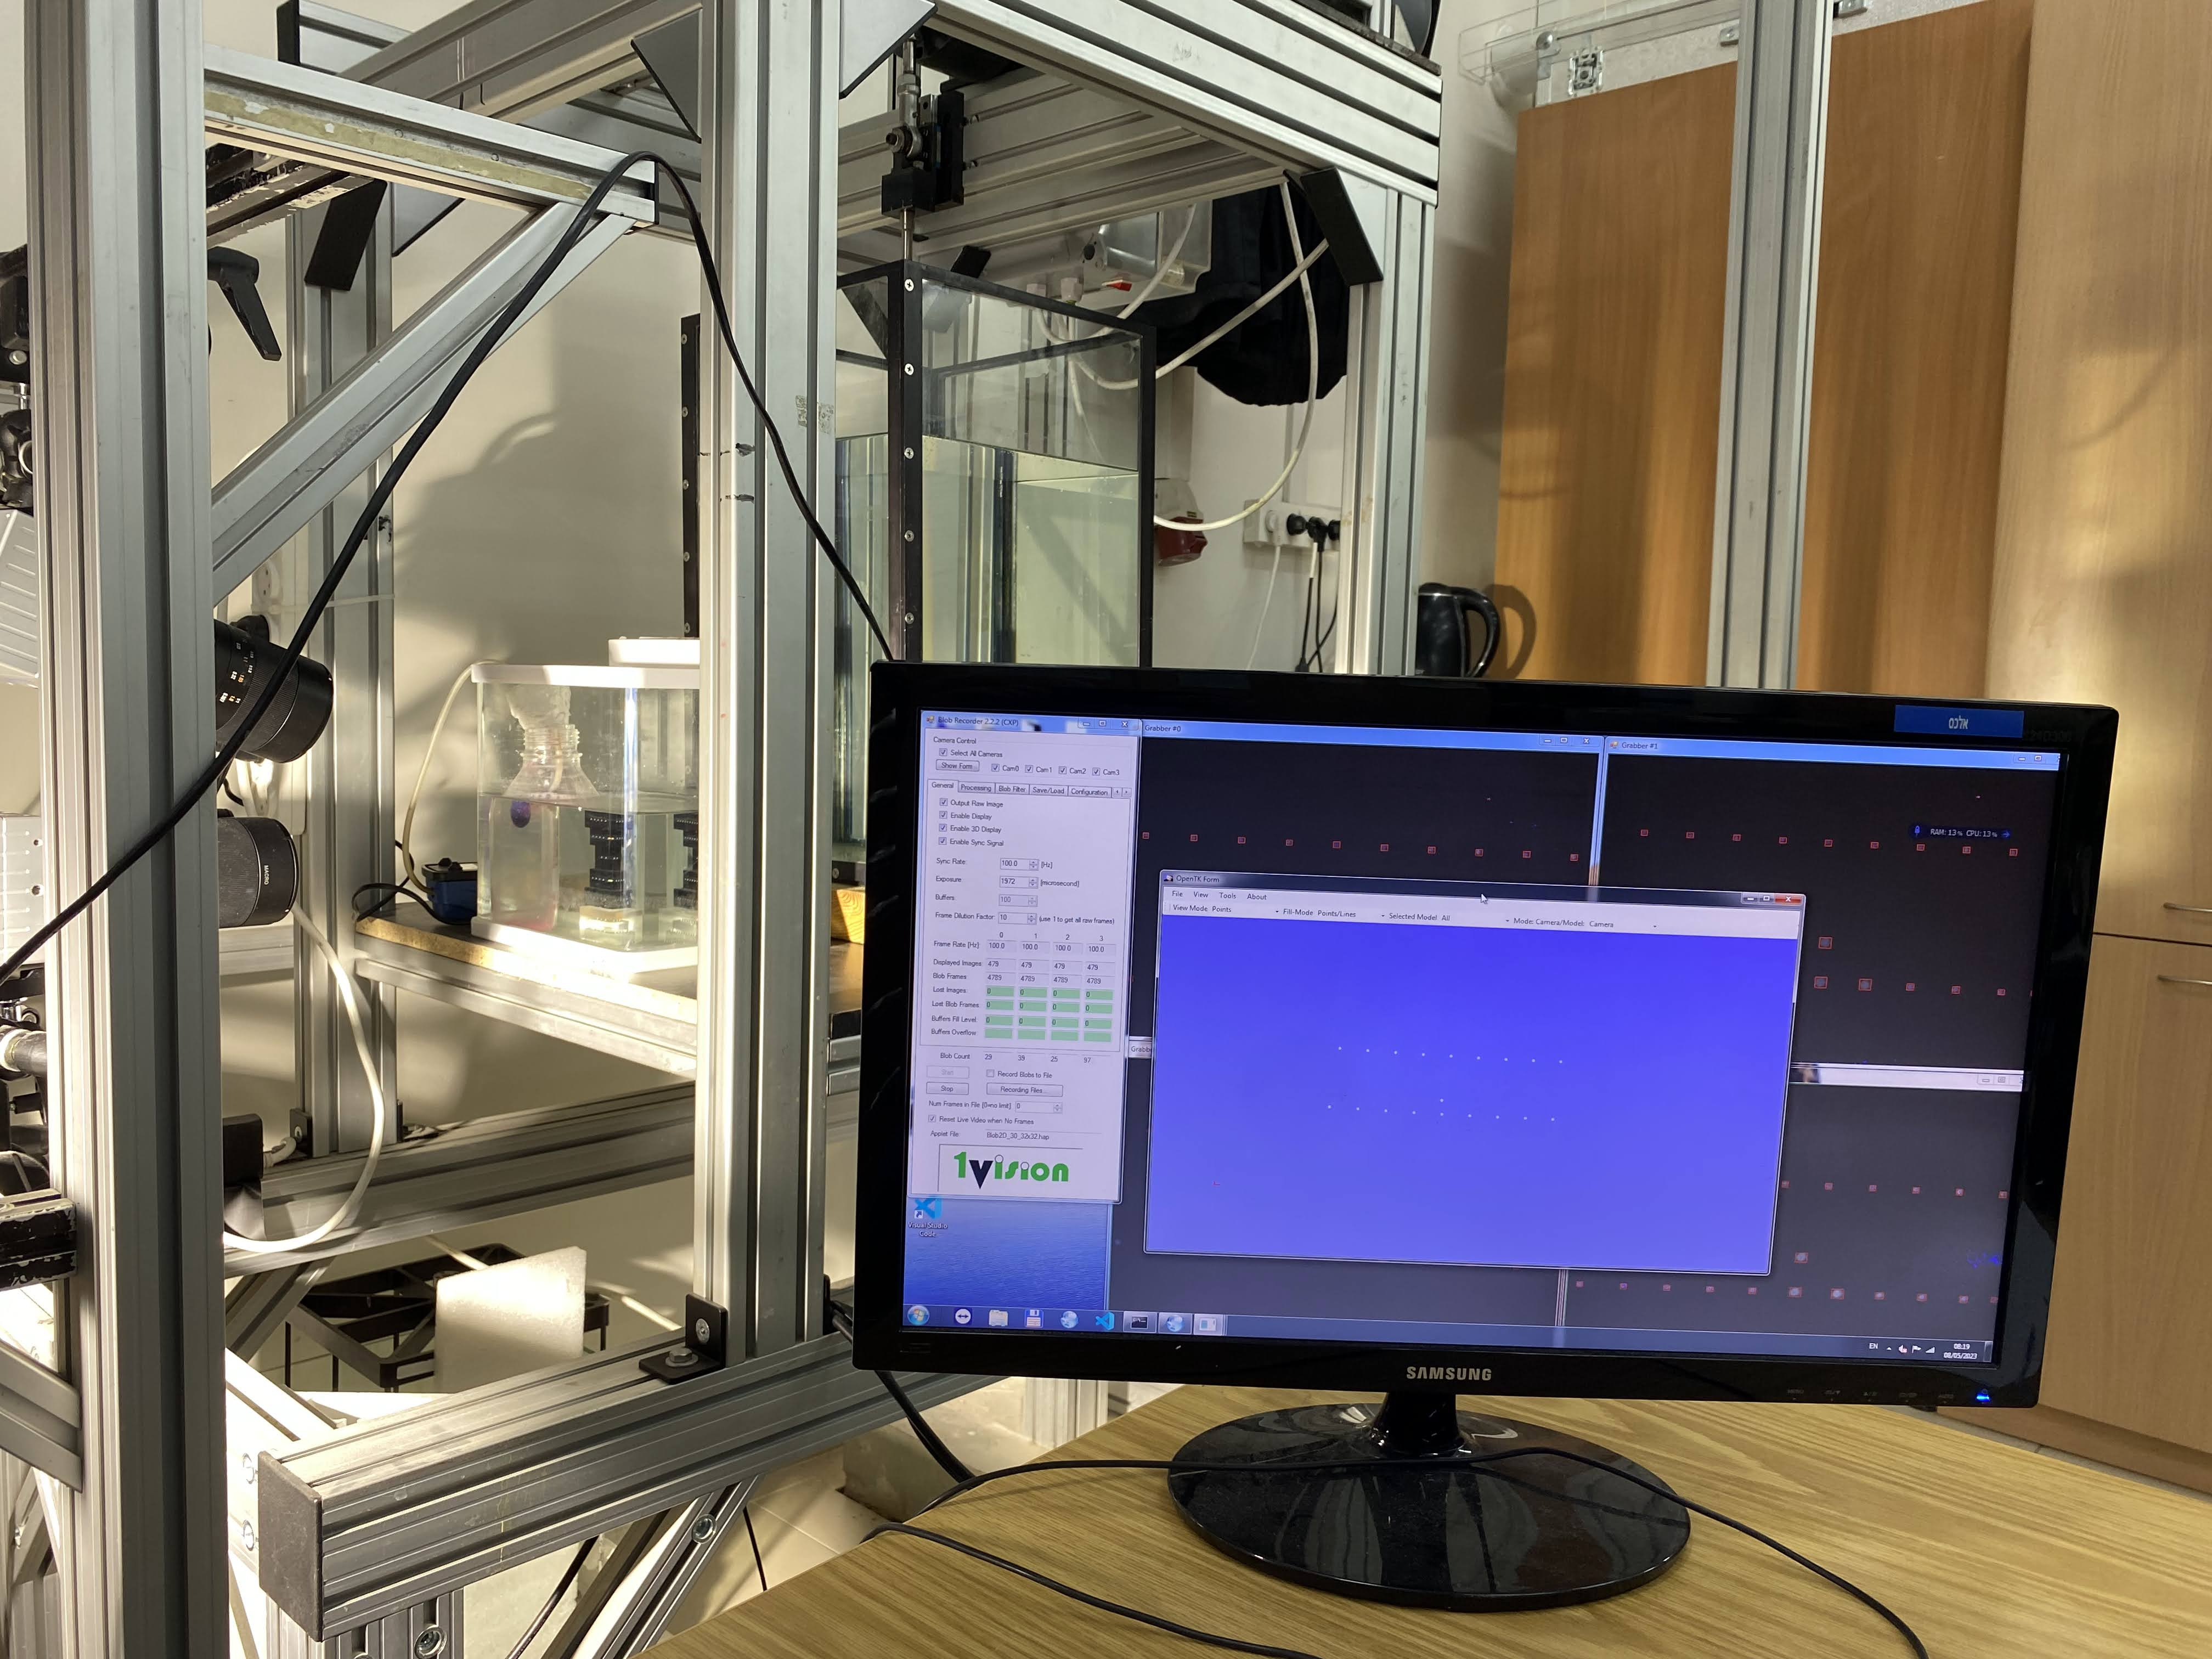
\includegraphics[width=0.9\textwidth]{fig/real_time_3dptv_snapshot.jpg}}{video/real_time_3dptv.mp4}    
  \end{frame}



% \subsection{Credits}
\topicFramePrimary{Credits}

\begin{frame}[label=credit-1a]{The credit goes to the collaborators and funding agencies}
\begin{multicols}{2}
\centering
\cardImg{group_photo.jpg}{.49\textwidth} \cardImg{calibration_team.jpg}{0.49\textwidth}
\cardImg{sabrina_caliper.jpg}{.49\textwidth}\cardImg{meny_sabrina.jpg}{0.49\textwidth}
\end{multicols}
\end{frame}
